% Template using the rsuqreport class for producing standard reports from the Chair of Risk, Safety 
% and Uncertainty Quantification in ETH Zurich.
% Copyright 2013, Stefano Marelli and Bruno Sudret, all rights reserved. 
% Please contact Stefano Marelli (marelli@ibk.baug.ethz.ch) for any template-related enquiries.
\documentclass{rsuqreport}

% additional packages/package options may be added here


% % % % % % % % % % % % % % % % % % % % % % % % % % % % % % % % % % % % % % % % % % % % % % % % % %
% THE FOLLOWING INFORMATION NEEDS TO BE PROVIDED TO PROPERLY COMPILE THE REPORT INTESTATION. 	  %
% PLEASE NOTE THAT THE FIELDS CAN BE LEFT EMPTY, BUT THEY MUST NOT BE REMOVED!					  %
% % % % % % % % % % % % % % % % % % % % % % % % % % % % % % % % % % % % % % % % % % % % % % % % % %

% Report title. Due to restriction on the template design, please make sure it is at most 3 lines 
% long
\title{RSUQ Report Template}
% List of authors (comma separated) as it will appear on the paper
\author{Ann Author, Another Author}

% Name of the client the report is addressed to
\clientname{Enterprise Inc.}
% Identifier for the contract
\contractref{Research Agreement n$^\circ$ AB12345}
% Contact person for the client
\contactname{Dr. G. Freeman}
% Address of the client (Can be multi-line text)
\clientaddress{	Stefano-Franscini-Platz 5\\ 
				CH-8093 Z\"urich\\
				Switzerland }
% ETH Project number related to the report
\ethprojectnum{312345}
% Reference name for the report
\reportref{R-312345-001/A/}



% Abstract of the report. May contain any type of formatting
\reportabstract{
	Lorem ipsum dolor sit amet, consectetuer adipiscing elit. Ut purus
	elit, vestibulum ut, placerat ac, adipiscing vitae, felis. Curabitur
	dictum gravida mauris. Nam arcu libero, nonummy eget, consectetuer id,
	vulputate a, magna. Donec vehicula augue eu neque. Pellentesque
	habitant morbi tristique senectus et netus et malesuada fames ac
	turpis egestas. Mauris ut leo. Cras viverra metus rhoncus sem. Nulla
	et lectus vestibulum urna fringilla ultrices.  Phasellus eu tellus sit
	amet tortor gravida placerat. Integersapien est, iaculis in, pretium
	quis, viverra ac, nunc. Praesent eget sem vel leo ultrices bibendum.
	Aenean faucibus. Morbi dolor nulla, malesuada eu, pulvinar at, mollis
	ac, nulla.  Curabitur auctor semper nulla. Donec varius orci eget
	risus. Duis nibh mi, congue eu, accumsan eleifend, sagittis quis,
	diam. Duis eget orci sit amet orci dignissim rutrum.
	
	Nam dui ligula, fringilla a, euismod sodales, sollicitudin vel, wisi.
	Morbi auctor lorem non justo. Nam lacus libero, pretium at, lobortis
	vitae, ultricies et, tellus. Donec aliquet, tortor sed accumsan biben-
	dum, erat ligula aliquet magna, vitae ornare odio metus a mi. Morbi ac
	orci et nisl hendrerit mollis. Suspendisse ut massa. Cras nec ante.
	Pellentesque a nulla. Cum sociis natoque penatibus et magnis dis
	parturient montes, nascetur ridiculus mus. Aliquam tincidunt urna.
	Nulla ullamcorper vestibulum turpis. Pellentesque cursus luctus
	mauris.
	
}
\keywords{Lorem, ipsum}

% BEGINNING OF THE REAL DOCUMENT CONTENTS

\begin{document}


\section{First Section}
\subsection{Subsection}
\subsubsection{Subsubsection}
TARATATATA

Nulla malesuada porttitor diam. Donec felis erat, congue non, volutpat
at, tincidunt tristique, libero. Vivamus viverra fermentum felis.
Donec nonummy pellentesque ante. Phasellus adipiscing semper elit.
Proin fermentum massa ac quam. Sed diam turpis, molestie vitae,
placerat a, molestie nec, leo. Maecenas lacinia. Nam ipsum ligula,
eleifend at, accumsan nec, suscipit a, ipsum. Morbi blandit ligula
feugiat magna. Nunc eleifend consequat lorem. Sed lacinia nulla vitae
enim. Pellentesque tincidunt purus vel magna.  Integer non enim.
Praesent euismod nunc eu purus. Donec bibendum quam in tellus.  Nullam
cursus pulvinar lectus. Donec et mi. Nam vulputate metus eu enim.
Vestibulum pellentesque felis eu massa.

\begin{equation}
E = mc^2
\label{eqn: Einstein}
\end{equation}

Quisque ullamcorper placerat ipsum. Cras nibh. Morbi vel justo vitae
lacus tincidunt ultrices. Lorem ipsum dolor sit amet, consectetuer
adipiscing elit. In hac habitasse platea dictumst. Integer tempus
convallis augue. Etiam facilisis.  Nunc elementum fermentum wisi.
Aenean placerat. Ut imperdiet, enim sed gravida sollicitudin, felis
odio placerat quam, ac pulvinar elit purus eget enim. Nunc vitae
tortor. Proin tempus nibh sit amet nisl. Vivamus quis tortor vitae
risus porta vehicula.



\subsection{Table}
This is a sample table referred to as Table \ref{table: random variables}
\begin{table}[h]
	\centering

	\begin{tabular}{cccc}
		\hline
		Parameter & Distribution & Mean & Coefficient of variation \\ \hline
		    L     &  Lognormal   &  1m  &           3\%            \\
		    b     &  Lognormal   & 10cm &           3\%            \\
		    h     &  Lognormal   & 1cm  &           3\%            \\ \hline
	\end{tabular}
	\caption{Example of a table}
	\label{table: random variables}
	
\end{table}

\section{Figures}
This is a sample figure referred to as Figure \ref{img: test figure}.
\begin{figure}[h!]
	\centering
	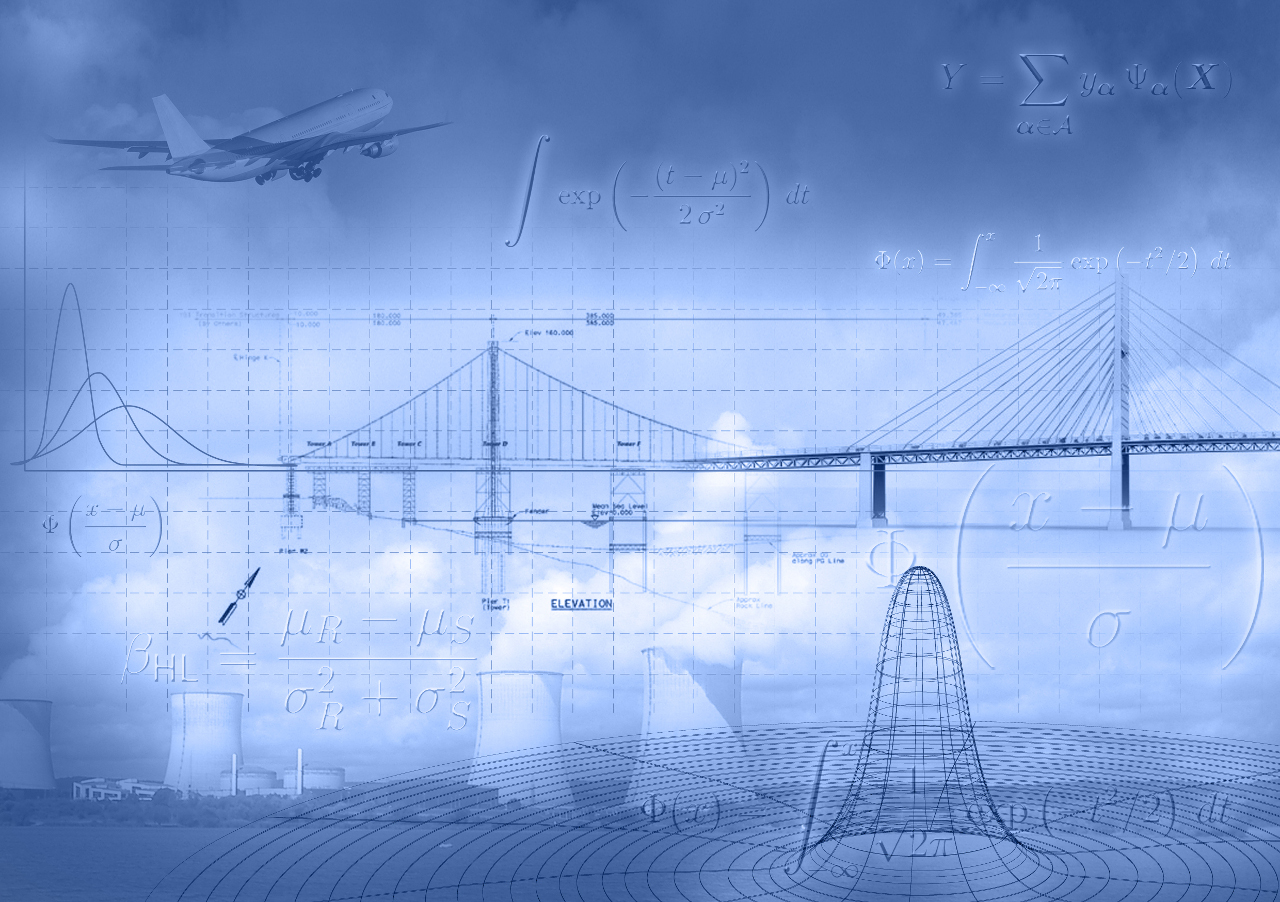
\includegraphics[width = .3\textwidth]{ReportBackGround_75dpi_1MP.jpg}
	\caption{This is a sample figure}
	\label{img: test figure}
\end{figure}


\section{Notation}
A set of standard notation is defined in the file \verb|bstnotation.sty| and shall be 
used 
whenever justified.

\section{References}
Citations are managed with \textsc{Bib}\TeX. A data base (\eg{} \verb|test.bib|) iis 
used to gather 
all the bibliography. All papers of interest shall be stored in this \verb|bib| file.

In order to use it, the commands \verb|\citep| and \verb|\citet| from the 
\verb|natbib| package are 
used:
\begin{itemize}
\item If the citation appears \emph{within} a sentence, it is referred to using 
\verb|\citet|, as 
in:  
	\begin{itemize}
		\item[] \citet{Bourinet2011} introduced support vector machines and subset 
		simulation in 
		order to compute small probabilities of failure
	\end{itemize}
\item If the citation appears \emph{at the end} of the sentence, \ie{} using 
parenthesis, the 
\verb|\citep| command shall be used, as in:\\
\begin{itemize}
	\item[] The use of support vector machines for structural reliability analysis was 
	proposed 
		recently \citep{Bourinet2011,Basudhar2008a,Basudhar2008b}.
\end{itemize}
\end{itemize}

\bibliographystyle{chicago}
\bibliography{testbib}

\end{document}

